% Glossareinträge
\newacronym{cpu}{CPU}{Central Processing Unit}
\newglossaryentry{Ampere}
{
  name=Ampere,
  description={die SI-Basiseinheit der elektrischen Stromstärke}
}
\newglossaryentry{gpio}
{
  name=GPIO,
  description={General Purpose Input/Output\newline Kontakte, die Softwareseitig für verschiedene Zwecke angesteuert werden können\newline z.B.: Auslesen von Sensoren, Ansteuern von Displays}
}

% Ende Glossareinträge

\chapter{Hardware}

Die Hardware besteht aus einem Raspberry Pi, \todo{genauere Beschreibung}
\section{Der Raspberry Pi}
\begin{wrapfigure}{r}{0.5\textwidth}
 \vspace{-16pt}
 \centering 
 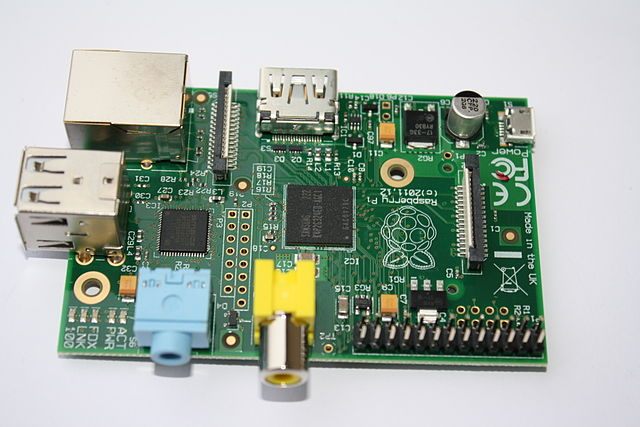
\includegraphics[width=0.45\textwidth]{figures/raspberry.jpg}
 \caption[Raspberry Pi - Modell B]{Raspberry Pi - Modell B\footnotemark}
 \vspace{-50pt}
\end{wrapfigure}
\footnotetext{\cite{rasp_bild}}
Der \textit{Raspberry Pi} ist ein Einplatinencomputer, der 2012 von der  \textit{Raspberry Pi Foundation} auf den Markt gebracht wurde. 
\subsection{Geschichte}
Ursprünglich war er als günstiger Computer gedacht, um britischen Jugendlichen das Programmieren näher zu bringen. An der \textit{University of Cambridge} stellte man fest, dass die Vorkenntnisse von Studienanfängern immer geringer wurden, weil sie -- sowohl privat als auch in der Schule -- sich immer weniger mit der Funktionsweise von Computern und Programmen beschäftigen. Daher wollte man einen Computer entwickeln, mit dem die Jugendlichen experimentieren können.
\footcite{aboutraspberry}$^,$\todo{absolut geschummelt}
\footcite{wiki:raspi_geschichte}

\subsection{Technische Daten}
Die Technik in einem Raspberry Pi ist vergleichbar mit der eines Smartphones. Der Raspberry Pi hat eine \acrshort{cpu} mit 700 MHz, welche auf bis zu 1 GHz übertaktbar ist, und je nach Modell 256 oder 512 MB Arbeitsspeicher. Als Speichermedium für das Betriebssystem (verschiedene Linux-Distributionen stehen zur Auswahl) wird eine SD-Karte bzw. eine microSD-Karte verwendet.

Zur Stromversorgung genügt ein normales Handy-Ladegerät mit Micro-USB-Anschluss und 1 \gls{Ampere} Stromstärke, denn der Raspberry Pi benötigt nur 3,5 Watt\footcite{strom} (Modell B).

Zum Anschließen anderer Hardware gibt es zwei USB-Anschlüsse und 26 \gls{gpio}-Pins.

\section{Sensoren}
Zur Messung der Werte werden folgende Sensoren verwendet:
\begin{itemize}
\item 4 Temperatursensoren \textit{DS18B20}
\item Luftfeuchtesensor \textit{DHT22}
\item Luftdrucksensor \textit{BMP085}
\item Luftqualitätssensor \textit{VOLTCRAFT CO-20}
\item CPU-Temperatur des Raspberry Pi
\end{itemize}
\subsection{Temperatur}
Mithilfe der Temperatursensoren werden die Innentemperatur, die Gehäusetemperatur und die Bodentemperatur (Außen) gemessen. Der hat eine Messgenauigkeit von $\pm 0.5\degree C$  und einen Messbereich von $-10\degree C$ bis $+85\degree C$. \footcite[20]{temp}

